\begin{frame}[t]{Distribution}
  \vspace{0.6cm}
  \begin{center}
    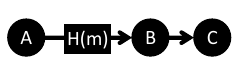
\includegraphics[width=0.50\textwidth]{logic}
  \end{center}
  \begin{itemize}
  \item A programm consists of logical stages (A, B, C)
  \item connected with a connector (H(m)) which controls exchange of data between stages
  \end{itemize}
\end{frame}

\begin{frame}[t]{Distribution}
  \vspace{0.15cm}
   \begin{center}
   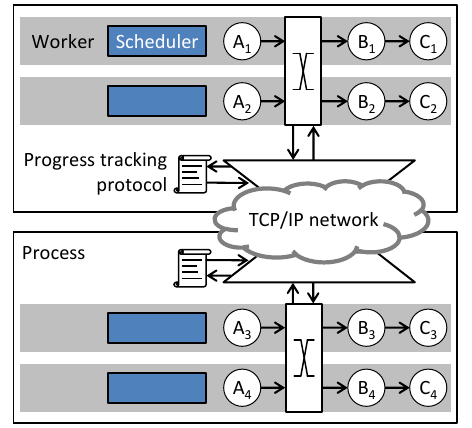
\includegraphics[height=0.4\textwidth]{physical}
   \end{center}
   \begin{itemize}
     \item physical graph represents the chosen amount of workers and distirbuted connected hosts
     \item programmer can selected which way a message should flow in the system
stages
\item Naiad always uses the logical graph as a decision base where data has to flow
    \end{itemize}

\end{frame}

\begin{frame}[t]{Worker}
  \vspace{0.15cm}
delivers message (data) and notifications (done with epoch) to vertices

   \begin{itemize}
     \item data gets always delivered before notifications
     \item is responsible for multiple vertexes
	 \item loop data does not pass trough the workers queue
   \end{itemize}

\end{frame}

\begin{frame}[t]{Progress tracking}
  \vspace{0.15cm}
\textbf{Problem}: notificaion can only be send if there are no outstanding messages

\textbf{Solution}: own progress tracking protocol
   \begin{itemize}
     \item Occurence Counters gets updated after a Broadcast (with progress update) to all workers
     \item Local counter never moves ahead of global counter
	 \item Allows save deliverance of notification
   \end{itemize}

\end{frame}

\begin{frame}[t]{Optimation progress update}
  \vspace{0.15cm}
   \begin{itemize}
     \item rely on the logical graph and not the physical one
     \item buffer before broadcast
	 \item optimistically first broadcast via UDP to reduce latency
     \item programming primitives which allow threads to be woken by either a broadcast or unicast
   \end{itemize}

\end{frame}

 \begin{frame}[t]{Fault tolerance and availability}
  \vspace{0.15cm}
  CHECKPOINT and RESTORE interface
   \begin{itemize}
     \item Vertex
	 \begin{itemize}
	 	\item either log data or
        \item full checkpoint when requested
	 \end{itemize}
     \item Progress Tracking Protocoll
     \begin{itemize}
     	\item full checkpoint
     \end{itemize}
   \end{itemize}

\end{frame}


 \begin{frame}[t]{}
  \vspace{0.15cm}
Tradeoff between Performance and Durability
   \begin{itemize}
     \item paper favours performance over durablity
     \item Prelies on durable input and output
   \end{itemize}

\end{frame}

 \begin{frame}[t]{Micro strugglers}
  \vspace{0.15cm}
Naiad is sensitive to latency but tiny interruptions can decrease overall performance  

\begin{tabular}{ l r }
  Iterative Computation & $$<$$ 1 MS \\
  GC, Package loss   & 10th of MS \\
\end{tabular}

Network

\begin{itemize}
\item Disable Nagle's algorithms
\item Set smaller retry timeout for package loss
\item Use different network protocols in datacenters for computing
\end{itemize}

Garbage Collection

\begin{itemize}
\item avoid object allocation
\item use buffer pools
\item use value types
\end{itemize}

\end{frame}

 \begin{frame}[t]{Naiad programm}
  \vspace{0.15cm}
   \begin{itemize}
     \item public API with primitives
     \item higher Level APIs
     \begin{itemize}
     \item LINQ
     \item MapReduce
     \item Pregel
     \end{itemize}
     \item examples does not support coordination
     \begin{itemize}
     \item to improve performance
     \item for Example concat, distinct, select
     \end{itemize}
     \item API for vertex programming
     \begin{itemize}
     \item first define the behavior dataflow vertices
     \item second define the topology
     \end{itemize}
   \end{itemize}

\end{frame}
